\chapter{Factorización prima}\label{chapter:factorizacionPrima}

\section{Teorema Fundamental de la Aritmética}\label{section_TFA}
\rule{\textwidth}{0.1mm}
\begin{act}
	Mediante un programa decir si un número es primo o no, luego encontrar los números primos menores que 100 o entre un rango dado.
\end{act}
\rule{\textwidth}{0.1mm}

\textbf{Cuántos números primos existen?}\\


Todo número puede ser factorizado en factores primos, por ejemplo $30=2\cdot3\cdot5$. Cuando aparece más veces un factor primo usamos las potencias, por ejemplo $375=3^1\cdot5^3$.\\

\textbf{Hay algún número que no se pueda descomponer en factores primos?}\\
\textbf{Hay dos números que tengan la misma descomposición en factores primos?}\\

\begin{theorem} \textbf{(Teorema Fundamental de la Aritmética)}\\
	Todo número entero positivo tiene exactamente una única factorización prima. Es decir, dado $a\in {\mathbb{Z}}^{+}$, se tiene que existe una única factorización prima:
	\[a={p_1}^{\alpha_1} \cdot {p_2}^{\alpha_2} \cdot {p_3}^{\alpha_3} \cdots {p_n}^{\alpha_n} \]
\end{theorem}

\textbf{OJO. } Todo número en su descomposición contiene a todos los números primos. Por ejemplo
\[
		375=2^{\color{red}0}\color{black}\cdot 3^1\cdot5^3\cdot 7^{\color{red}0}\color{black}\cdot 11^{\color{red}0}\color{black}\cdot 13^{\color{red}0}\color{black}\cdot 17^{\color{red}0}\color{black}\cdots
\]
\rule{\textwidth}{0.1mm}
\begin{act}
	Mediante un programa hacer la descomposición prima de un número.
\end{act}
\rule{\textwidth}{0.1mm}


\section{Multiplos y MCM}\label{section_multiplos_MCM}
Analicemos los múltiplos en una descomposición prima. 
\begin{center}
\begin{itemize}
	\item $45=\color{red} 3^2\cdot 5^1$
	\item $90=2^1\cdot \color{red} 3^2\cdot 5^1$
	\item $135=3\cdot \color{red} 3^2\cdot 5^1 \color{black}= \color{red} 3^{\color{black}3 }\cdot\color{red} 5^1$
	\item $180=2^2\cdot \color{red} 3^2\cdot 5^1$
\end{itemize}
\end{center}

\textbf{OJO. }La factorización de $mn$, contiene la factorización de $n$ y $m$\\
\textbf{Denotaremos: }$m.c.m\{a,b\}=[a,b]$\\

\begin{ejemplo}
	Encontrar el mínimo común múltiplo de 12 y 45. \\
	\textit{\textbf{Rta:} $[12,45]$ va a ser un número que contiene la factorización de 12 y la de 45, pues es múltiplo de ambos y además es el más pequeño posible. Como $12=\color{blue}2^2\cdot 3^1$ y $45=\color{red}3^2\cdot 5^1$ entonces $[12,45]=\color{blue}2^2\cdot\color{red}3^2\cdot 5^1=\color{black}180$}.
	
	Podemos hallar múltiplos de 180 y así ir encontrando todos los múltiplos comunes de 12 y 45.
\end{ejemplo}

\newpage
\begin{exers}{\ \\}
	\begin{center}
		\vspace{-1cm}
		\subsubsection*{ Mínimo común múltiplo }\label{ejercicios_subsubsection_MCM}
	\end{center}

	\begin{enumerate}
	\item (4.3.1 de \cite{Aops_TN}). Usando la factorización prima encontrar:
				\begin{enumerate}[label=\Alph*)]
					\item $[42,72]$
					\item $[10,56]$
					\item $[9,12,16]$		
				\end{enumerate}
	\item (4.3.3 de \cite{Aops_TN}). Encontrar los primeros 6 múltiplos comunes más pequeños entre 14,15 y 16.
	\item (4.3.4 de \cite{Aops_TN}). Encontrar el menor número de 4 dígitos que sea divisible por 2,3,4,5,6 y 7.
	
	
	\end{enumerate}
\end{exers}
\newpage


Es importante saber hacer y usar la factorización prima, pues esta nos permitirá manipular los enteros para resolver algunos problemas de una forma más rápida. 

\begin{prop}\textbf{(Mínimo común múltiplo)}\\
Dados dos números $a={p_1}^{\alpha_1} \cdot {p_2}^{\alpha_2} \cdot {p_3}^{\alpha_3} \cdots {p_n}^{\alpha_n}$ y $b={p_1}^{\beta_1} \cdot {p_2}^{\beta_2} \cdot {p_3}^{\beta_3} \cdots {p_n}^{\beta_n}$
\[
[a,b]= {p_1}^{\max\{\alpha_1,\beta_1\}} \cdot {p_2}^{\max\{\alpha_1,\beta_1\}} \cdot {p_3}^{\max\{\alpha_1,\beta_1\}} \cdots {p_n}^{\max\{\alpha_1,\beta_1\}}
\]
\end{prop}


\section{Divisores y MCD}\label{section_Divisores_y_MCD}

Así como la factorización permite encontrar los múltiplos, también permite encontrar los divisores.

\begin{ejemplo}\label{Ejemplo_aopsTN_4_11}
	(4.11 de \cite{Aops_TN}). Encontrar la factorización prima de 60 y ver cómo los divisores están relacionados con ella. \\
	\textit{\textbf{Rta:} Podemos ver que $60=2^2\cdot3^1\cdot 5^1$. Por ejemplo 12 es divisor pues $12=\color{red}2^2\cdot 3^1\cdot 5^0$ y $60=\color{red}2^2\cdot 3^1\color{black} \cdot 5^1$}. De la misma forma podemos ver que
		\begin{figure}[H]
			\centering
			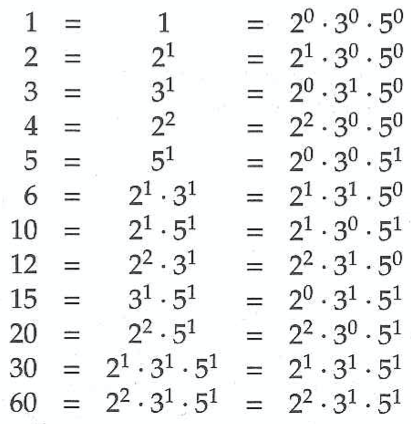
\includegraphics[width=0.35\linewidth]{TN/imgs/4_11_aops_tn}
			\caption{Ejemplo \ref{Ejemplo_aopsTN_4_11}}
			\label{4_11_aops_tn}
		\end{figure}
\end{ejemplo}

\textbf{OJO. }La factorización de $n$, contiene la factorización de los divisores de $n$\\
\textbf{Denotaremos: }$m.c.d\{a,b\}=(a,b)$\\

\begin{ejemplo}\label{Ejemplo_aopsTN_4_13}
	Encontrar el máximo  común divisor de 36 y 84. \\
	\textit{\textbf{Rta:} $(36,84)$ va a ser un número que está en la factorización de 36 y en la de 84, pues es divisor de ambos y además es el más grande posible. Como $36=\color{blue}2^2\cdot 3^2$ y $84=\color{red}2^2\cdot 3^1\cdot 7^1$ entonces $(36,84)= 2^2\cdot3^1 =12$}.
	
	Podemos hallar los divisores de 12 y así encontrar todos los divisores comunes de 36 y 84:
	\begin{figure}[H]
		\centering
		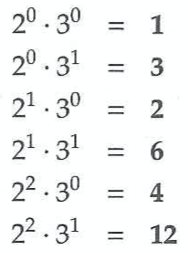
\includegraphics[width=0.2\linewidth]{TN/imgs/4_13_aops_tn}
		\caption{Ejemplo \ref{Ejemplo_aopsTN_4_13}}
		\label{4_13_aops_tn}
	\end{figure}
\end{ejemplo}

\newpage
\begin{exers}{\ \\}
	\begin{center}
		\vspace{-1cm}
		\subsubsection*{ Máximo común divisor }\label{ejercicios_subsubsection_MCD}
	\end{center}

	\begin{enumerate}
		\item (4.4.1 de \cite{Aops_TN}). Usando la factorización prima encontrar:
		\begin{enumerate}[label=\Alph*)]
			\item $(12,20)$
			\item $(140,320)$
		\end{enumerate}
		\item (4.4.2 de \cite{Aops_TN}). Encontrar los divisores comunes de 108 y 360.
	\end{enumerate}
\end{exers}
\newpage

\begin{prop}\textbf{(Máximo común divisor)}\\
	Dados dos números $a={p_1}^{\alpha_1} \cdot {p_2}^{\alpha_2} \cdot {p_3}^{\alpha_3} \cdots {p_n}^{\alpha_n}$ y $b={p_1}^{\beta_1} \cdot {p_2}^{\beta_2} \cdot {p_3}^{\beta_3} \cdots {p_n}^{\beta_n}$
	\[
	(a,b)= {p_1}^{\min\{\alpha_1,\beta_1\}} \cdot {p_2}^{\min\{\alpha_2,\beta_2\}} \cdot {p_3}^{\min\{\alpha_3,\beta_3\}} \cdots {p_n}^{\min\{\alpha_3,\beta_n\}}
	\]
\end{prop}

\section{Cuadrados y cubos perfectos}\label{section_cuadrados_cubos_perfectos}

\begin{ejemplo}
	Cómo es la factorización prima de un cuadrado perfecto?\\
	\textit{\textbf{Rta:} Ejemplo, la factorización de $12^2={(2^2\cdot 3^1)}^2=2^4\cdot 3^2$}.
		
	Cuáles de las siguientes descomposiciones son de un cuadrado perfecto? Si no lo son, cuál es el cuadrado perfecto mas grande que lo divide?
	\begin{enumerate}[label=\Alph*)]
	\item $2^8$. 
	\item $2\cdot3^2$. 
	\item $2^{10}\cdot3^2\cdot 5^3$.
	\item $2^2\cdot 7^2$.
	\end{enumerate}
\end{ejemplo}

\begin{ejemplo}
	Cómo es la factorización prima de un cubo perfecto?\\
	\textit{\textbf{Rta:} Ejemplo, la factorización de $18^3={(2^1\cdot 3^2)}^3=2^3\cdot 3^6$}.
	
	Cuáles de las siguientes descomposiciones son de un cubo perfecto? Si no lo son, cuál es el cubo perfecto mas grande que lo divide?
	\begin{enumerate}[label=\Alph*)]
		\item $2^8$. 
		\item $2^3\cdot3^1$. 
		\item $2^{9}\cdot3^3\cdot 5^{13}$.
		\item $2^6\cdot 7^9$.
	\end{enumerate}
\end{ejemplo}

\begin{ejemplo}
	Gina escribe los cubos de tres enteros positivos en un papel. Ricardo dice que cada uno es múltiplo de 18. Gina luego dice que el máximo común divisor de los tres cubos es $n$. Encontrar el valor más pequeño que $n$ puede tener.
\end{ejemplo}

\newpage
\begin{exers}{\ \\}
	\begin{center}
		\vspace{-1cm}
		\subsubsection*{ Descomposición de cuadrados y cubos perfectos }\label{ejercicios_subsubsection_cuadrados_y_cubos_perfectos}
	\end{center}

	
	\begin{enumerate}
		\item (4.6.1 de \cite{Aops_TN}). Encontrar los cinco cuadrados perfectos mas pequeños que son múltipos de 6.
		\item (4.6.3 de \cite{Aops_TN}). Encontrar los seis enteros mas pequeños que son cuadrados perfectos y cubos perfectos.	
		\item (4.6.4 de \cite{Aops_TN}). Encontrar los cuatro cubos perfectos mas pequeños que son múltiplos de 30.
		\item (4.6.5 de \cite{Aops_TN}). Carmelita escribe en una lista el cuadrado perfecto más pequeño que es múltiplo de 20,  el cubo perfecto más pequeño que es múltiplo de 20 y todos los múltiplos de 20 que están entre estos números. Cuántos números hay en la lista de Carmelita?
	\end{enumerate}
\end{exers}
\newpage

\section{Propiedades MCM y MCD}\label{section_propiedades_MCM_MCD}

\begin{ejemplo}\label{Ejemplo_aopsTN_4_20}
	Encontrar $(80n,144n)$ y $[80n,144n]$. \\
\textbf{Rta:} Por ejemplo para cuando $\textbf{n=2}$ tenemos que 
	\begin{equation*}
			\begin{split}
					\textbf{2}\cdot \color{blue} 80 \color{black} &= \textbf{2}\cdot\color{blue}(2^4\cdot3^0\cdot 5^1 )\color{black}=2^5\cdot 3^0\cdot 5^1 \\
					\textbf{2}\cdot \color{red} 144 \color{black}& =\textbf{2}\cdot\color{red}(2^4\cdot3^2\cdot 5^0 )\color{black} =2^5\cdot3^2\cdot 5^0,
			\end{split}
	\end{equation*}
entonces 
	\begin{equation*}
			\begin{split}
					(\textbf{2}\cdot \color{blue} 8\color{black},\textbf{2}\cdot \color{red} 144 \color{black})= 2^5\cdot3^0\cdot 5^0=\textbf{2}\cdot(\color{blue} 8\color{black}, \color{red} 144 \color{black}),
			\end{split}
	\end{equation*}
y
	\begin{equation*}
		\begin{split}
		[\textbf{2}\cdot \color{blue} 8\color{black},\textbf{2}\cdot \color{red} 144 \color{black}]= 2^5\cdot3^2\cdot 5^1=\textbf{2}\cdot[\color{blue} 8\color{black}, \color{red} 144 \color{black}].
		\end{split}
	\end{equation*}
Si hacemos lo mismo para $\textbf{n=3}$, podemos ver que 
	\begin{equation*}
	\begin{split}
	\textbf{3}\cdot \color{blue} 80 \color{black} &= \textbf{3}\cdot\color{blue}(2^4\cdot3^0\cdot 5^1 )\color{black}=2^4\cdot 3^1\cdot 5^1 \\
	\textbf{3}\cdot \color{red} 144 \color{black}& =\textbf{3}\cdot\color{red}(2^4\cdot3^2\cdot 5^0 )\color{black} =2^4\cdot3^3\cdot 5^0,
	\end{split}
	\end{equation*}
	entonces 
	\begin{equation*}
	\begin{split}
	(\textbf{3}\cdot \color{blue} 8\color{black},\textbf{3}\cdot \color{red} 144 \color{black})= 2^4\cdot3^1\cdot 5^0=\textbf{3}\cdot(\color{blue} 8\color{black}, \color{red} 144 \color{black}),
	\end{split}
	\end{equation*}
	y
	\begin{equation*}
	\begin{split}
	[\textbf{3}\cdot \color{blue} 8\color{black},\textbf{2}\cdot \color{red} 144 \color{black}]= 2^4\cdot3^3\cdot 5^1=\textbf{3}\cdot[\color{blue} 8\color{black}, \color{red} 144 \color{black}].
	\end{split}
	\end{equation*}
	Podemos hacerlo sucesivamente y ver que en general
		\begin{equation*}
		\begin{split}
		(\textbf{n}\cdot \color{blue} 8\color{black},\textbf{n}\cdot \color{red} 144 \color{black})=\textbf{n}\cdot(\color{blue} 8\color{black}, \color{red} 144 \color{black}),
		\end{split}
		\end{equation*}
		y
		\begin{equation*}
		\begin{split}
				[\textbf{n}\cdot \color{blue} 8\color{black},\textbf{n}\cdot \color{red} 144 \color{black}]=\textbf{n}\cdot[\color{blue} 8\color{black}, \color{red} 144 \color{black}],
		\end{split}
		\end{equation*}
\end{ejemplo}

\begin{exer}{\ \\}
	(4.21 de \cite{Aops_TN}). Encontrar  $(800,1800)$ y $[800,1800]$.
\end{exer}

\begin{prop}
Dados $a,b$ y $n$ enteros positivos se cumple que 
\begin{enumerate}
		\item $(n\cdot a,n\cdot b)= n\cdot (a,b)$
		\item $[n\cdot a,n\cdot b]= n\cdot [a,b]$		
\end{enumerate}
\end{prop}

\begin{prop}
	Dados $a$ y $b$ enteros positivos se cumple que 
	\[a\cdot b= (a,b)[a,b]\]
\end{prop}

\begin{proof}
	Si $a=P_1^{\alpha_1}\cdot P_2^{\alpha_2}\cdots P_n^{\alpha_n} $ y $b=P_1^{\beta_1}\cdot P_2^{\beta_2}\cdots P_n^{\beta_n} $, entonces 
	\begin{align*}
	(a,b)[a,b] 		&= {p_1}^{\min\{\alpha_1,\beta_1\}} \cdot {p_2}^{\min\{\alpha_2,\beta_2\}} \cdots {p_n}^{\min\{\alpha_n,\beta_n\}} \color{red}\cdot \color{black} {p_1}^{\max\{\alpha_1,\beta_1\}} \cdot {p_2}^{\max\{\alpha_2,\beta_2\}} \cdots {p_n}^{\max\{\alpha_n,\beta_n\}} \\
	&= {p_1}^{\min\{\alpha_1,\beta_1\}} \cdot {p_1}^{\max\{\alpha_1,\beta_1\}} \cdot {p_2}^{\min\{\alpha_2,\beta_2\}} {p_2}^{\max\{\alpha_2,\beta_2\}} \cdots {p_n}^{\min\{\alpha_n,\beta_n\}} \cdot {p_n}^{\max\{\alpha_n,\beta_n\}}\\
	&= {p_1}^{\min\{\alpha_1,\beta_1\} +  \max\{\alpha_1,\beta_1\} }\cdot {p_2}^{\min\{\alpha_2,\beta_2\} + \max\{\alpha_2,\beta_2\}}  \cdots {p_n}^{\min\{\alpha_n,\beta_n\} + \max\{\alpha_n,\beta_n\}} \\
	&= {p_1}^{\alpha_1 + \beta_1} \cdot {p_2}^{\alpha_2 + \beta_2} \cdots {p_n}^{\alpha_n+ \beta_n} \\
	&= P_1^{\alpha_1}\cdot P_1^{\beta_1} \cdot P_2^{\alpha_2}\cdot P_2^{\beta_2}\cdots P_n^{\alpha_n} \cdot P_n^{\beta_n}\\
	&= P_1^{\alpha_1}\cdot P_2^{\alpha_2}\cdots P_n^{\alpha_n} \color{red}\cdot \color{black}  P_1^{\beta_1}\cdot P_2^{\beta_2}\cdots P_n^{\beta_n}\\
	&= a\cdot b
	\end{align*}
\end{proof}












\begin{exer}{\ \\}
	(4.23 de \cite{Aops_TN}). Si el máximo común divisor entre 70 y $n$ es 10 y el mínimo común múltiplo es 210. Encontrar $n$.
\end{exer}

\newpage
\begin{exers}{\ \\}
	\begin{center}
		\vspace{-1cm}
		\subsubsection*{ Propiedades del MCM y MCD }\label{ejercicios_subsubsection_propiedades_de_MCM_MCD}
	\end{center}

	\begin{enumerate}
		\item (4.7.1 de \cite{Aops_TN}). De forma sencilla encontrar 
				\begin{enumerate}[label=\Alph*)]
						\item (50,90)
						\item (750,600)
						\item $[60,70]$
						\item $[444,555]$																		
				\end{enumerate}
		\item (4.7.2 de \cite{Aops_TN}). Encontrar el producto del máximo comun divisor y el mínimo común múltiplo de 100 y 120.
		\item (4.7.3 de \cite{Aops_TN}). Encontrar $n$ si $(n,40)=10$ y $[n,40]=240$.
		\item (4.7.4 de \cite{Aops_TN}). El máximo común divisor entre dos números es 6 y  el mínimo común múltiplo es 450. Si uno de los números es 18, cuál es el otro número?
	\end{enumerate}
\end{exers}
\newpage


\begin{exers}{\ \\}
	\begin{center}
		\vspace{-5mm}
		\section*{Ejercicios de revisión}\label{section_ejercicios_factorizacion_prima_MCM_MCD}
	\end{center}
	\begin{enumerate}
		\item (4.36 de \cite{Aops_TN}). Encontrar $(2520,720)$.
		\item (4.38 de \cite{Aops_TN}). El mínimo común múltiplo de 12,15,20 y $k$ es 420. Cuál es el valor mas pequeño posible que puede tener $k$?
		\item (4.39 de \cite{Aops_TN}). \textbf{Wow}. Un grupo de 10 amigos estan discutiendo sobre un número. ``El se puede dividir por 1" dice el primer amigo. ``El se puede dividir por 2" dice el segundo. ``El se puede dividir por 3" dice el tercero. ``El se puede dividir por 4" dice el cuarto. Continúan así hasta que los diez dicen su comentario.  Si exactamente dos amigos estaban equivocados y estos amigos hablaron de forma consecutiva, cuál es el menor número posible sobre el cuál estaban discutiendo?
		\item (4.40 de \cite{Aops_TN}). \textbf{Wow}. Cuál es el entero positivo $N$ más pequeño tal que el valor $7+30N$ no es un número primo?
		\item (4.41 de \cite{Aops_TN}). Encontrar los cinco múltiplos comunes más pequeños de 18 y 30 que sean cuadrados perfectos y cubos perfectos.				
		\item (4.42 de \cite{Aops_TN}). \textbf{Wow}. El producto de un conjunto de números es 140. Cuál es la suma más pequeña posible que estos pueden tener?		
		\item (4.43 de \cite{Aops_TN}). Encontrar el máximo entero positivo tal que sea divisor de cualquier múltiplo común de 14,26 y 66.
		\item (4.44 de \cite{Aops_TN}). Cuál de los siguientes números tiene el divisor propio más grande: 1999, 2000 o 2001? (Nota: los divisores propios de un número son los divisores sin incluir al mismo número)
		\item (4.45 de \cite{Aops_TN}). 	
						\begin{enumerate}[label=\Alph*)]
							\item Calcular $[24,90]$.
							\item Cualquier múltiplo de 24 y 90 es también múltiplo de 36?
							\item Cualquier múltiplo de 24 y 90 es también múltiplo de 2160?																	
						\end{enumerate}
		\item (4.46 de \cite{Aops_TN}). El más grande de dos números es 8 veces el otro. Explique por qué ambos no pueden ser a la vez cuadrados perfectos?
		\item (4.47 de \cite{Aops_TN}). La suma de los recíprocos de tres números consecutivos es $\frac{47}{60}$. Cuál es la suma de estos tres enteros?
		\item (4.49 de \cite{Aops_TN}). Cuál es el divisor primo más grande de la siguiente serie aritmética:\[1+2+3+\cdots +70?\]
		\item (4.50 de \cite{Aops_TN}). \textbf{Wow.} Encontrar el entero positivo más pequeño que deja residuo 1 cuando se divide por $2,3,\dots,8$ y 9. 
		\item (4.51 de \cite{Aops_TN}). Cuál es el entero positivo más pequeño que al ser multiplicado por 200 es un cubo perfecto?
		\item (4.52 de \cite{Aops_TN}). Juliana escribe los enteros desde 1 hasta 2000 en un papel. Ella borra todos los múltiplos de 3, luego los múltiplos de 5, y así sucesivamente, borrando todos los múltiplos de cada primo impar. Cuántos quedan luego de que termina ?
		\item (4.53 de \cite{Aops_TN}).\textbf{Wow. }Cuántos valores posibles tiene la suma $a+b+c$ si $a,b$ y $c$ son enteros positivos y $abc=72$?
		\item (4.54 de \cite{Aops_TN}). Alex cuenta hasta 400 de 6 en 6 y Mateo cuenta hasta 400 de 4 en 4. Cuántos de los números contados por Alex fueron también contados por Mateo?
		\item (4.55 de \cite{Aops_TN}). Cualquier producto entre dos de los números 30,72 y $N$ es divisible por el tercero. Cuál es el valor mas pequeño posibile que puede tener $N$?
		\item Encontrar todas las parejas de enteros positivos $n$ y $m$ tales que $(n,m)=6$ y $[n,m]=600$.
		
		\item (4.57 de \cite{Aops_TN}). \textbf{Wow}. Bruno, Fernando y Valentina están jugando un juego donde cada carta tiene el número $2,3,4,5,6,7$ o 8. Cada uno se pone la carta en su frente de modo que solo los demás la pueden ver. Juan va caminando y observa que los tres números no son todos diferentes y además que su producto es un cuadrado perfecto. Cuántos de los tres jugadores pueden ahora deducir el número en su frente? 
		
		\item (Selectiva UIS Nivel medio 2020). De los divisores de $5^6\times 7^8$ cuántos son cuadrados perfectos?
		
	\end{enumerate}
\end{exers}
\newpage

\chapter{Divisores: contando divisores, producto de divisores.}\label{chapter:contandoDivisores}

\section{Contando divisores }\label{section:contandoDivisores}


\newpage
\begin{exers}{\ \\}
	\begin{center}
		\vspace{-1cm}
		\subsubsection*{ Contando Dividores }\label{ejercicios:contandoDivisores}
	\end{center}
	
	\begin{enumerate}
		\item (Selectiva UIS Nivel Avanzado 2020). El número \textbf{abab} tiene exactamente 14 divisores. Cuál es el valor de $a+2b$?
		
	\end{enumerate}
\end{exers}
\newpage


\section{Producto de divisores }\label{section:productoDeDivisores}